%=================================================================
% Chương 2 - Cơ sở lý thuyết của phân tích tách biệt tuyến tính
% File này là nội dung chương/tiểu mục để chèn vào luận văn bằng \input{}
% Nếu dùng như tài liệu độc lập, hãy thêm preamble phù hợp trong file main.
%=================================================================
\chapter{Phân tích tách biệt tuyến tính}

Trong các bài toán phân loại mẫu thống kê, đối tượng quan sát thường được biểu diễn dưới dạng một vectơ đặc trưng nhiều chiều $x \in \mathbb{R}^d$. Mỗi quan sát thuộc về một trong $K$ lớp $c_1,c_2,\ldots,c_K$, và mục tiêu của bài toán là xây dựng một quy tắc quyết định để từ một mẫu mới có thể xác định lớp của nó một cách chính xác nhất. Khi số chiều của dữ liệu lớn, việc phân loại trực tiếp trong không gian gốc thường gặp nhiều khó khăn do cấu trúc dữ liệu phức tạp, khả năng trực quan hóa hạn chế, và nguy cơ tồn tại những biến không thật sự hữu ích cho việc phân biệt lớp.

Phân tích tách biệt tuyến tính (Linear Discriminant Analysis -- LDA) là một trong những phương pháp kinh điển của thống kê nhiều chiều cho cả hai mục tiêu: \emph{giảm chiều có giám sát} và \emph{phân loại}. Điều đáng chú ý là LDA có thể được hiểu từ hai góc nhìn khác nhau nhưng thống nhất ở kết quả cuối cùng. Góc nhìn thứ nhất là cách tiếp cận của Fisher, trong đó ta tìm một phép chiếu tuyến tính sao cho dữ liệu sau khi chiếu tách biệt lớp tốt nhất. Góc nhìn thứ hai là lý thuyết quyết định Bayes, trong đó quy tắc phân loại tối ưu được xây dựng từ xác suất hậu nghiệm; dưới giả thiết Gaussian với cùng ma trận hiệp phương sai, quy tắc Bayes dẫn đến một bộ phân loại tuyến tính. Chính sự gặp nhau của hai hướng tiếp cận này tạo nên nền tảng lý thuyết hoàn chỉnh của LDA.

Vì vậy, để hiểu đầy đủ phương pháp LDA, chương này sẽ trình bày lần lượt ba nội dung chính. Trước hết là cách tiếp cận của Fisher với tiêu chuẩn tối đa hóa sự tách biệt giữa các lớp. Tiếp theo là cơ sở của lý thuyết quyết định Bayes trong bài toán phân loại. Cuối cùng, trên nền tảng Bayes, ta chỉ ra cách mô hình Gaussian với ma trận hiệp phương sai chung dẫn trực tiếp đến LDA, đồng thời cho thấy sự tương đương giữa hướng nhìn xác suất và hướng nhìn hình học.

\section{Phương pháp tách biệt tuyến tính của Fisher}

\subsection{Ý tưởng hình học của Fisher}

Khác với lý thuyết Bayes, Fisher không khởi đầu bằng một mô hình xác suất đầy đủ cho từng lớp. Ông xuất phát từ một câu hỏi mang tính hình học: nếu dữ liệu đã có nhãn lớp, có thể tìm được một phép chiếu tuyến tính sao cho sau khi chiếu, các lớp được tách biệt tốt nhất hay không? Trong trường hợp hai lớp, Fisher tìm một vectơ $\beta$ để chiếu dữ liệu từ không gian $\mathbb{R}^d$ xuống một trục một chiều:
\begin{equation}
Z = \beta^T X.
\end{equation}

Sau phép chiếu này, mỗi lớp sẽ có một trung bình và một mức độ phân tán riêng trên trục $Z$. Một hướng chiếu tốt là hướng làm khoảng cách giữa các trung bình lớp trên trục chiếu càng lớn càng tốt, đồng thời làm phương sai trong từng lớp trên trục chiếu càng nhỏ càng tốt.

Giả sử có quần thể hai lớp $l={C_{1},C_{2}}$
\begin{itemize}
    \item Lớp $C_{1}$ với phân phối dữ liệu $X_{1}$.
    \item Lớp $C_{2}$ với phân phối dữ liệu $X_{2}$.
\end{itemize}
Mỗi quan sát $\bm{x}\in \mathbb{R}^d$ sao cho chiếu dữ liệu xuống một trục sao cho 'hai lớp cách xa nhau nhất' hay 'ít chồng lấn nhất'

\begin{figure}[h] % h: tại đây, t: đầu trang, b: cuối trang, p: trang riêng
    \centering % Căn giữa hình ảnh
    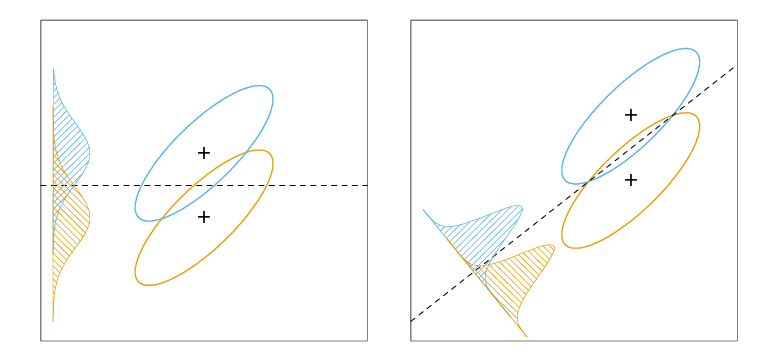
\includegraphics[width=0.8\textwidth]{image/image_1_Fisher_idea.png} 
    \caption{Ý tưởng hình học của Fisher để phân tách hai lớp tốt nhất} % Nội dung hiện dưới hình
    \label{fig:hinh1} % Dùng để trích dẫn bằng lệnh \ref{fig:hinh1}
\end{figure}
\textbf{Nhận xét}
\begin{itemize}
    \item Khoảng cách giữa các tâm của hai lớp sau khi chiếu phải lớn nhất.
    \item Độ tản mát (phương sai) của dữ liệu trong nội bộ mỗi lớp sau khi chiếu phải nhỏ nhất, nghĩa là dữ liệu co cụm lại.
\end{itemize}

\subsection{Cơ sở lý thuyết theo LDA của Fisher}

\subsubsection{Ma trận tán xạ trong lớp và giữa các lớp}

Để lượng hóa hai ý tưởng ``cách xa nhau nhất giữa các lớp'' và ``tụ lại ở trong lớp'', Fisher đưa vào hai đại lượng cơ bản.

Với mỗi lớp $C_{k}$, gọi $\mu_k$ là vectơ trung bình mẫu của lớp đó. Ma trận tán xạ trong lớp được xác định bởi
\begin{equation}
S_W = \sum_{k=1}^{K}\sum_{x_i \in C_k}(x_i-\mu_k)(x_i-\mu_k)^T.
\end{equation}

Ma trận này mô tả độ phân tán của các điểm quanh trung bình lớp tương ứng. Nếu các điểm trong từng lớp tập trung lại gần nhau thì $S_W$ nhỏ; ngược lại, nếu dữ liệu phân tán rộng thì $S_W$ lớn.

Gọi $\mu$ là trung bình toàn cục của toàn bộ dữ liệu. Ma trận tán xạ giữa cáclớp được xác định bởi
\begin{equation}
S_B = \sum_{k=1}^{K} n_k(\mu_k-\mu)(\mu_k-\mu)^T,
\end{equation}
trong đó $n_k$ là số mẫu của lớp $k$. Ma trận này phản ánh mức độ phân tách giữa các lớp thông qua vị trí tương đối của các trung bình lớp so với trung bình toàn cục.

\subsection{Tiêu chuẩn Fisher trong bài toán hai lớp}

Trong trường hợp hai lớp, Fisher xét biến chiếu $Z=a^T X$. Gọi $m_1=a^T\mu_1$ và $m_2=a^T\mu_2$ là trung bình của hai lớp sau chiếu. Khi đó, độ tách biệt giữa hai lớp trên trục chiếu có thể đo bằng $(m_1-m_2)^2$. Đồng thời, phương sai trong lớp sau chiếu là
\begin{equation}
s_W^2 = a^T S_W a.
\end{equation}

Do đó, tiêu chuẩn Fisher được viết thành
\begin{equation}
J(a)=\frac{(a^T(\mu_1-\mu_2))^2}{a^T S_W a}.
\end{equation}

Đây là dạng hai lớp của tiêu chuẩn tổng quát
\begin{equation}
J(a)=\frac{a^T S_B a}{a^T S_W a}.
\end{equation}

Mục tiêu là tìm $a \neq 0$ sao cho $J(a)$ đạt cực đại.

\subsection{Nghiệm tối ưu của Fisher trong trường hợp hai lớp}

Đặt $m=\mu_1-\mu_2$, khi đó
\begin{equation}
J(a)=\frac{(a^T m)^2}{a^T S_W a}.
\end{equation}

Giả sử $S_W$ xác định dương. Đặt tiếp
\begin{equation}
b=S_W^{1/2}a, \qquad a=S_W^{-1/2}b.
\end{equation}
Suy ra
\begin{equation}
a^T m = b^T S_W^{-1/2}m
\end{equation}
và
\begin{equation}
a^T S_W a = b^T b.
\end{equation}
Do đó
\begin{equation}
J(a)=\frac{\bigl(b^T S_W^{-1/2}m\bigr)^2}{b^T b}.
\end{equation}

Áp dụng bất đẳng thức Cauchy--Schwarz,
\begin{equation}
\bigl(b^T S_W^{-1/2}m\bigr)^2 \le (b^T b)\bigl(m^T S_W^{-1}m\bigr).
\end{equation}
Suy ra
\begin{equation}
J(a)\le m^T S_W^{-1}m.
\end{equation}

Dấu bằng xảy ra khi và chỉ khi $b$ cùng phương với $S_W^{-1/2}m$, tức là
\begin{equation}
b=c\,S_W^{-1/2}m
\end{equation}
với một hằng số $c\neq 0$. Từ đó
\begin{equation}
a=S_W^{-1/2}b
= c\,S_W^{-1}m
= c\,S_W^{-1}(\mu_1-\mu_2).
\end{equation}

Vậy hướng chiếu tối ưu là
\begin{equation}
a \propto S_W^{-1}(\mu_1-\mu_2).
\end{equation}

Đây là công thức quan trọng nhất của Fisher trong bài toán hai lớp. Nó cho thấy hướng phân biệt tốt nhất không chỉ là hướng nối hai trung bình lớp, mà còn được điều chỉnh bởi cấu trúc phân tán trong lớp thông qua $S_W^{-1}$.

\subsection{Mở rộng cho nhiều lớp}

Trong trường hợp $K>2$, ta không còn tìm chỉ một hướng chiếu mà tìm một không gian con có số chiều thấp hơn, sao cho thông tin phân biệt giữa các lớp được giữ lại tốt nhất. Khi đó, bài toán quy về hệ trị riêng tổng quát
\begin{equation}
S_B a = \lambda S_W a,
\end{equation}
hay tương đương
\begin{equation}
S_W^{-1}S_B a = \lambda a,
\end{equation}
nếu $S_W$ khả nghịch. Các vectơ riêng ứng với các trị riêng lớn nhất tạo thành các trục phân biệt tối ưu.

\section{Lý thuyết quyết định Bayes trong bài toán phân loại}

\subsection{Xác suất hậu nghiệm và quy tắc Bayes tối ưu}

Trong lý thuyết quyết định thống kê, một quy tắc phân loại được xem là tối ưu nếu nó làm cực tiểu hóa rủi ro kỳ vọng. Trong trường hợp đơn giản nhất, khi chi phí phân loại đúng bằng $0$ và chi phí phân loại sai bằng $1$, bài toán tối ưu tương đương với việc cực tiểu hóa xác suất sai phân loại. Khi đó, quy tắc Bayes cho biết: với một quan sát $x$, ta nên gán $x$ vào lớp có xác suất hậu nghiệm lớn nhất. Nếu ký hiệu $G$ là biến ngẫu nhiên chỉ lớp, thì quy tắc này có dạng
\begin{equation}
G(x)=\arg\max_k P(G=k\mid X=x).
\end{equation}

Theo công thức Bayes,
\begin{equation}
P(G=k\mid X=x)=\frac{f_k(x)\pi_k}{\sum_{\ell=1}^{K}f_\ell(x)\pi_\ell},
\end{equation}
trong đó $f_k(x)=p(x\mid G=k)$ là mật độ có điều kiện của $X$ trong lớp $k$, còn $\pi_k=P(G=k)$ là xác suất tiên nghiệm của lớp đó. Vì mẫu số là như nhau cho mọi lớp khi so sánh, quy tắc Bayes tối ưu có thể viết gọn thành
\begin{equation}
G(x)=\arg\max_k \{f_k(x)\pi_k\}.
\end{equation}

Điều này cho thấy, nếu biết đầy đủ các mật độ lớp và các xác suất tiên nghiệm, thì bài toán phân loại về nguyên tắc đã được giải quyết.

\subsection{Mô hình Gaussian cho các lớp}

Để biến quy tắc Bayes thành một bộ phân loại cụ thể, cần giả thiết dạng của các mật độ lớp. Một giả thiết quan trọng trong thống kê nhiều chiều là mỗi lớp tuân theo phân phối chuẩn nhiều chiều. Cụ thể, với lớp $\omega_k$, ta giả sử
\begin{equation}
X\mid G=k \sim N_p(\mu_k,\Sigma_k),
\end{equation}
trong đó $\mu_k$ là vectơ trung bình và $\Sigma_k$ là ma trận hiệp phương sai của lớp $k$. Khi đó, mật độ lớp có dạng
\begin{equation}
f_k(x)=\frac{1}{(2\pi)^{p/2}|\Sigma_k|^{1/2}}
\exp\left\{-\frac12(x-\mu_k)^T\Sigma_k^{-1}(x-\mu_k)\right\}.
\end{equation}

Thay biểu thức này vào quy tắc Bayes và lấy logarit, ta thu được các hàm phân biệt
\begin{equation}
\delta_k(x)= -\frac12\log |\Sigma_k|
-\frac12(x-\mu_k)^T\Sigma_k^{-1}(x-\mu_k)
+\log \pi_k,
\end{equation}
bỏ qua các hằng số chung không phụ thuộc vào $k$. Khi đó, quy tắc phân loại Bayes trở thành
\begin{equation}
G(x)=\arg\max_k \delta_k(x).
\end{equation}

Nếu các $\Sigma_k$ khác nhau giữa các lớp, biên quyết định giữa hai lớp nói chung là bậc hai, và bộ phân loại nhận được là Quadratic Discriminant Analysis (QDA).

\section{LDA trong cách tiếp cận của lý thuyết quyết định Bayes}

\subsection{Trường hợp hiệp phương sai chung và sự xuất hiện của biên tuyến tính}

LDA xuất hiện như một trường hợp riêng có ý nghĩa đặc biệt của mô hình Gaussian ở trên, khi giả sử tất cả các lớp có chung một ma trận hiệp phương sai:
\begin{equation}
\Sigma_1=\Sigma_2=\cdots=\Sigma_K=\Sigma.
\end{equation}

Trong trường hợp này, các hàm phân biệt được rút gọn thành
\begin{equation}
\delta_k(x)=x^T\Sigma^{-1}\mu_k-\frac12\mu_k^T\Sigma^{-1}\mu_k+\log \pi_k.
\end{equation}

Công thức này cho thấy $\delta_k(x)$ là một hàm tuyến tính theo $x$. Do đó, biên quyết định giữa hai lớp bất kỳ $k$ và $\ell$, xác định bởi điều kiện $\delta_k(x)=\delta_\ell(x)$, có dạng
\begin{equation}
x^T\Sigma^{-1}(\mu_k-\mu_\ell)
-\frac12\bigl(\mu_k^T\Sigma^{-1}\mu_k-\mu_\ell^T\Sigma^{-1}\mu_\ell\bigr)
+\log\frac{\pi_k}{\pi_\ell}=0.
\end{equation}

Đây là phương trình của một siêu phẳng trong không gian $\mathbb{R}^p$. Như vậy, dưới giả thiết Gaussian nhiều chiều với cùng ma trận hiệp phương sai, quy tắc Bayes tối ưu cho phân loại là tuyến tính.

Trong trường hợp hai lớp $\omega_1$ và $\omega_2$, nếu đặt
\begin{equation}
a=\Sigma^{-1}(\mu_1-\mu_2)
\end{equation}
và
\begin{equation}
b=-\frac12\bigl(\mu_1^T\Sigma^{-1}\mu_1-\mu_2^T\Sigma^{-1}\mu_2\bigr)+\log\frac{\pi_1}{\pi_2},
\end{equation}
thì biên quyết định có dạng
\begin{equation}
a^T x+b=0.
\end{equation}

\subsection{Quy tắc phân loại LDA trong thực hành}

Trong thực tế, các tham số quần thể $\pi_k,\mu_k,\Sigma$ không biết trước và phải được ước lượng từ dữ liệu huấn luyện. Gọi $N$ là tổng số mẫu, $N_k$ là số mẫu thuộc lớp $k$. Các ước lượng tự nhiên được dùng trong LDA là
\begin{equation}
\hat \pi_k=\frac{N_k}{N}, \qquad
\hat \mu_k=\frac{1}{N_k}\sum_{g_i=k}x_i,
\end{equation}
và ma trận hiệp phương sai chung gộp
\begin{equation}
\hat \Sigma=
\frac{1}{N-K}
\sum_{k=1}^{K}\sum_{g_i=k}(x_i-\hat\mu_k)(x_i-\hat\mu_k)^T.
\end{equation}

Từ đó, các hàm phân biệt ước lượng có dạng
\begin{equation}
\hat\delta_k(x)=x^T\hat\Sigma^{-1}\hat\mu_k
-\frac12\hat\mu_k^T\hat\Sigma^{-1}\hat\mu_k
+\log\hat\pi_k,
\end{equation}
và quy tắc phân loại là
\begin{equation}
\hat G(x)=\arg\max_k \hat\delta_k(x).
\end{equation}

Trong bài toán hai lớp, điều này tương đương với việc kiểm tra dấu của hiệu $\hat\delta_1(x)-\hat\delta_2(x)$.

\subsection{Sự tương đương giữa Fisher và LDA theo Bayes}

Đến đây có thể thấy rằng hai cách tiếp cận tưởng như khác nhau thực ra dẫn đến cùng một cấu trúc toán học. Theo quyết định Bayes, dưới giả thiết Gaussian đồng hiệp phương sai, hướng quyết định giữa hai lớp phụ thuộc vào vectơ
\begin{equation}
\Sigma^{-1}(\mu_1-\mu_2).
\end{equation}

Theo Fisher, hướng chiếu tối ưu cho hai lớp là
\begin{equation}
S_W^{-1}(\mu_1-\mu_2).
\end{equation}

Trong mô hình Gaussian với hiệp phương sai chung, $S_W$ chỉ là ước lượng mẫu của cấu trúc phân tán trong lớp, còn $\Sigma$ là ma trận hiệp phương sai quần thể. Vì vậy, hai vectơ trên là cùng phương. Nói cách khác, hướng chiếu tối ưu của Fisher chính là hướng pháp tuyến của siêu phẳng Bayes trong trường hợp Gaussian đồng hiệp phương sai. Đây là kết luận nền tảng cho sự thống nhất giữa hai cách hiểu của LDA.

\subsection{Diễn giải bằng phép làm trắng và không gian phân biệt}

Một diễn giải hữu ích là xem LDA như quá trình \emph{làm trắng} dữ liệu theo hiệp phương sai chung rồi phân loại theo trọng tâm lớp. Nếu $\Sigma=\hat U\hat D\hat U^T$ là phân rã riêng của ma trận hiệp phương sai chung ước lượng, ta đặt
\begin{equation}
X^*=\hat D^{-1/2}\hat U^T X.
\end{equation}

Trong không gian mới, hiệp phương sai chung trở thành ma trận đơn vị. Khi đó, phân loại Bayes theo LDA tương đương với việc gán một điểm về trọng tâm lớp gần nhất trong không gian đã được làm trắng, có điều chỉnh thêm theo $\log \pi_k$ khi các xác suất tiên nghiệm khác nhau.

Một hệ quả quan trọng khác là trong LDA nhiều lớp, không gian phân biệt thực sự có số chiều tối đa là $K-1$. Sau khi làm trắng theo hiệp phương sai trong lớp, ta chỉ cần xét không gian con sinh bởi các trọng tâm lớp; không gian này chứa toàn bộ thông tin cần thiết cho phân loại LDA. Từ đó, bài toán reduced-rank LDA xuất hiện một cách tự nhiên thông qua việc phân rã riêng trên ma trận tán xạ giữa lớp trong không gian đã làm trắng.

\section{Quan hệ với QDA và một số mở rộng}

Nếu bỏ giả thiết các lớp có cùng ma trận hiệp phương sai, ta thu được bộ phân loại Bayes bậc hai, tức QDA. Khi đó, các hàm phân biệt có dạng
\begin{equation}
\delta_k(x)= -\frac12\log |\Sigma_k|
-\frac12(x-\mu_k)^T\Sigma_k^{-1}(x-\mu_k)
+\log \pi_k,
\end{equation}
và biên quyết định giữa các lớp là các mặt bậc hai.

Một hướng trung gian giữa LDA và QDA là Regularized Discriminant Analysis (RDA), trong đó
\begin{equation}
\hat\Sigma_k(\alpha)=\alpha\hat\Sigma_k+(1-\alpha)\hat\Sigma,
\qquad 0\le \alpha \le 1.
\end{equation}
Khi $\alpha=0$, ta quay về LDA; khi $\alpha=1$, ta thu được QDA.

\section{Kết luận}

Từ toàn bộ các phân tích trên, có thể rút ra rằng LDA là một phương pháp có nền tảng lý thuyết rất hoàn chỉnh. Ở góc độ hình học, LDA là lời giải của bài toán Fisher: tìm một phép chiếu tuyến tính sao cho tán xạ giữa lớp lớn nhất so với tán xạ trong lớp. Ở góc độ xác suất, LDA xuất hiện như bộ phân loại Bayes tối ưu khi dữ liệu của các lớp tuân theo phân phối Gaussian nhiều chiều với cùng ma trận hiệp phương sai. Hai con đường này gặp nhau ở cùng một hướng phân biệt.

Do đó, LDA không chỉ là một thuật toán phân loại mà còn là một phương pháp giảm chiều có giám sát rất tự nhiên, đồng thời là ví dụ điển hình cho sự thống nhất giữa tư duy tối ưu hình học và tư duy xác suất trong thống kê nhiều chiều.